% Chapter 7

\chapter{Multi-lable Classification Experiment} % Write in your own chapter title
\label{Chapter7}
\lhead{Chapter 7. \emph{Approach of Multi-label}}

\section{Artificial Dataset}

To demonstrate the approach, the dataset, named color detector, is created artificially. To each image, it has three labels for representing colour, $red$, $yellow$ and $blue$. If an image is red hue, it has a label for $red$ and label values of $yellow$ and $blue$ are negative. The representation of colour combination follows colour wheels. If an image has a hue close to $green$, it has positive labels for $yellow$ and $blue$, and negative label for $red$, and so on.
\graphicspath{ {./Figures/} }
\begin{figure}[!htb]
\centering
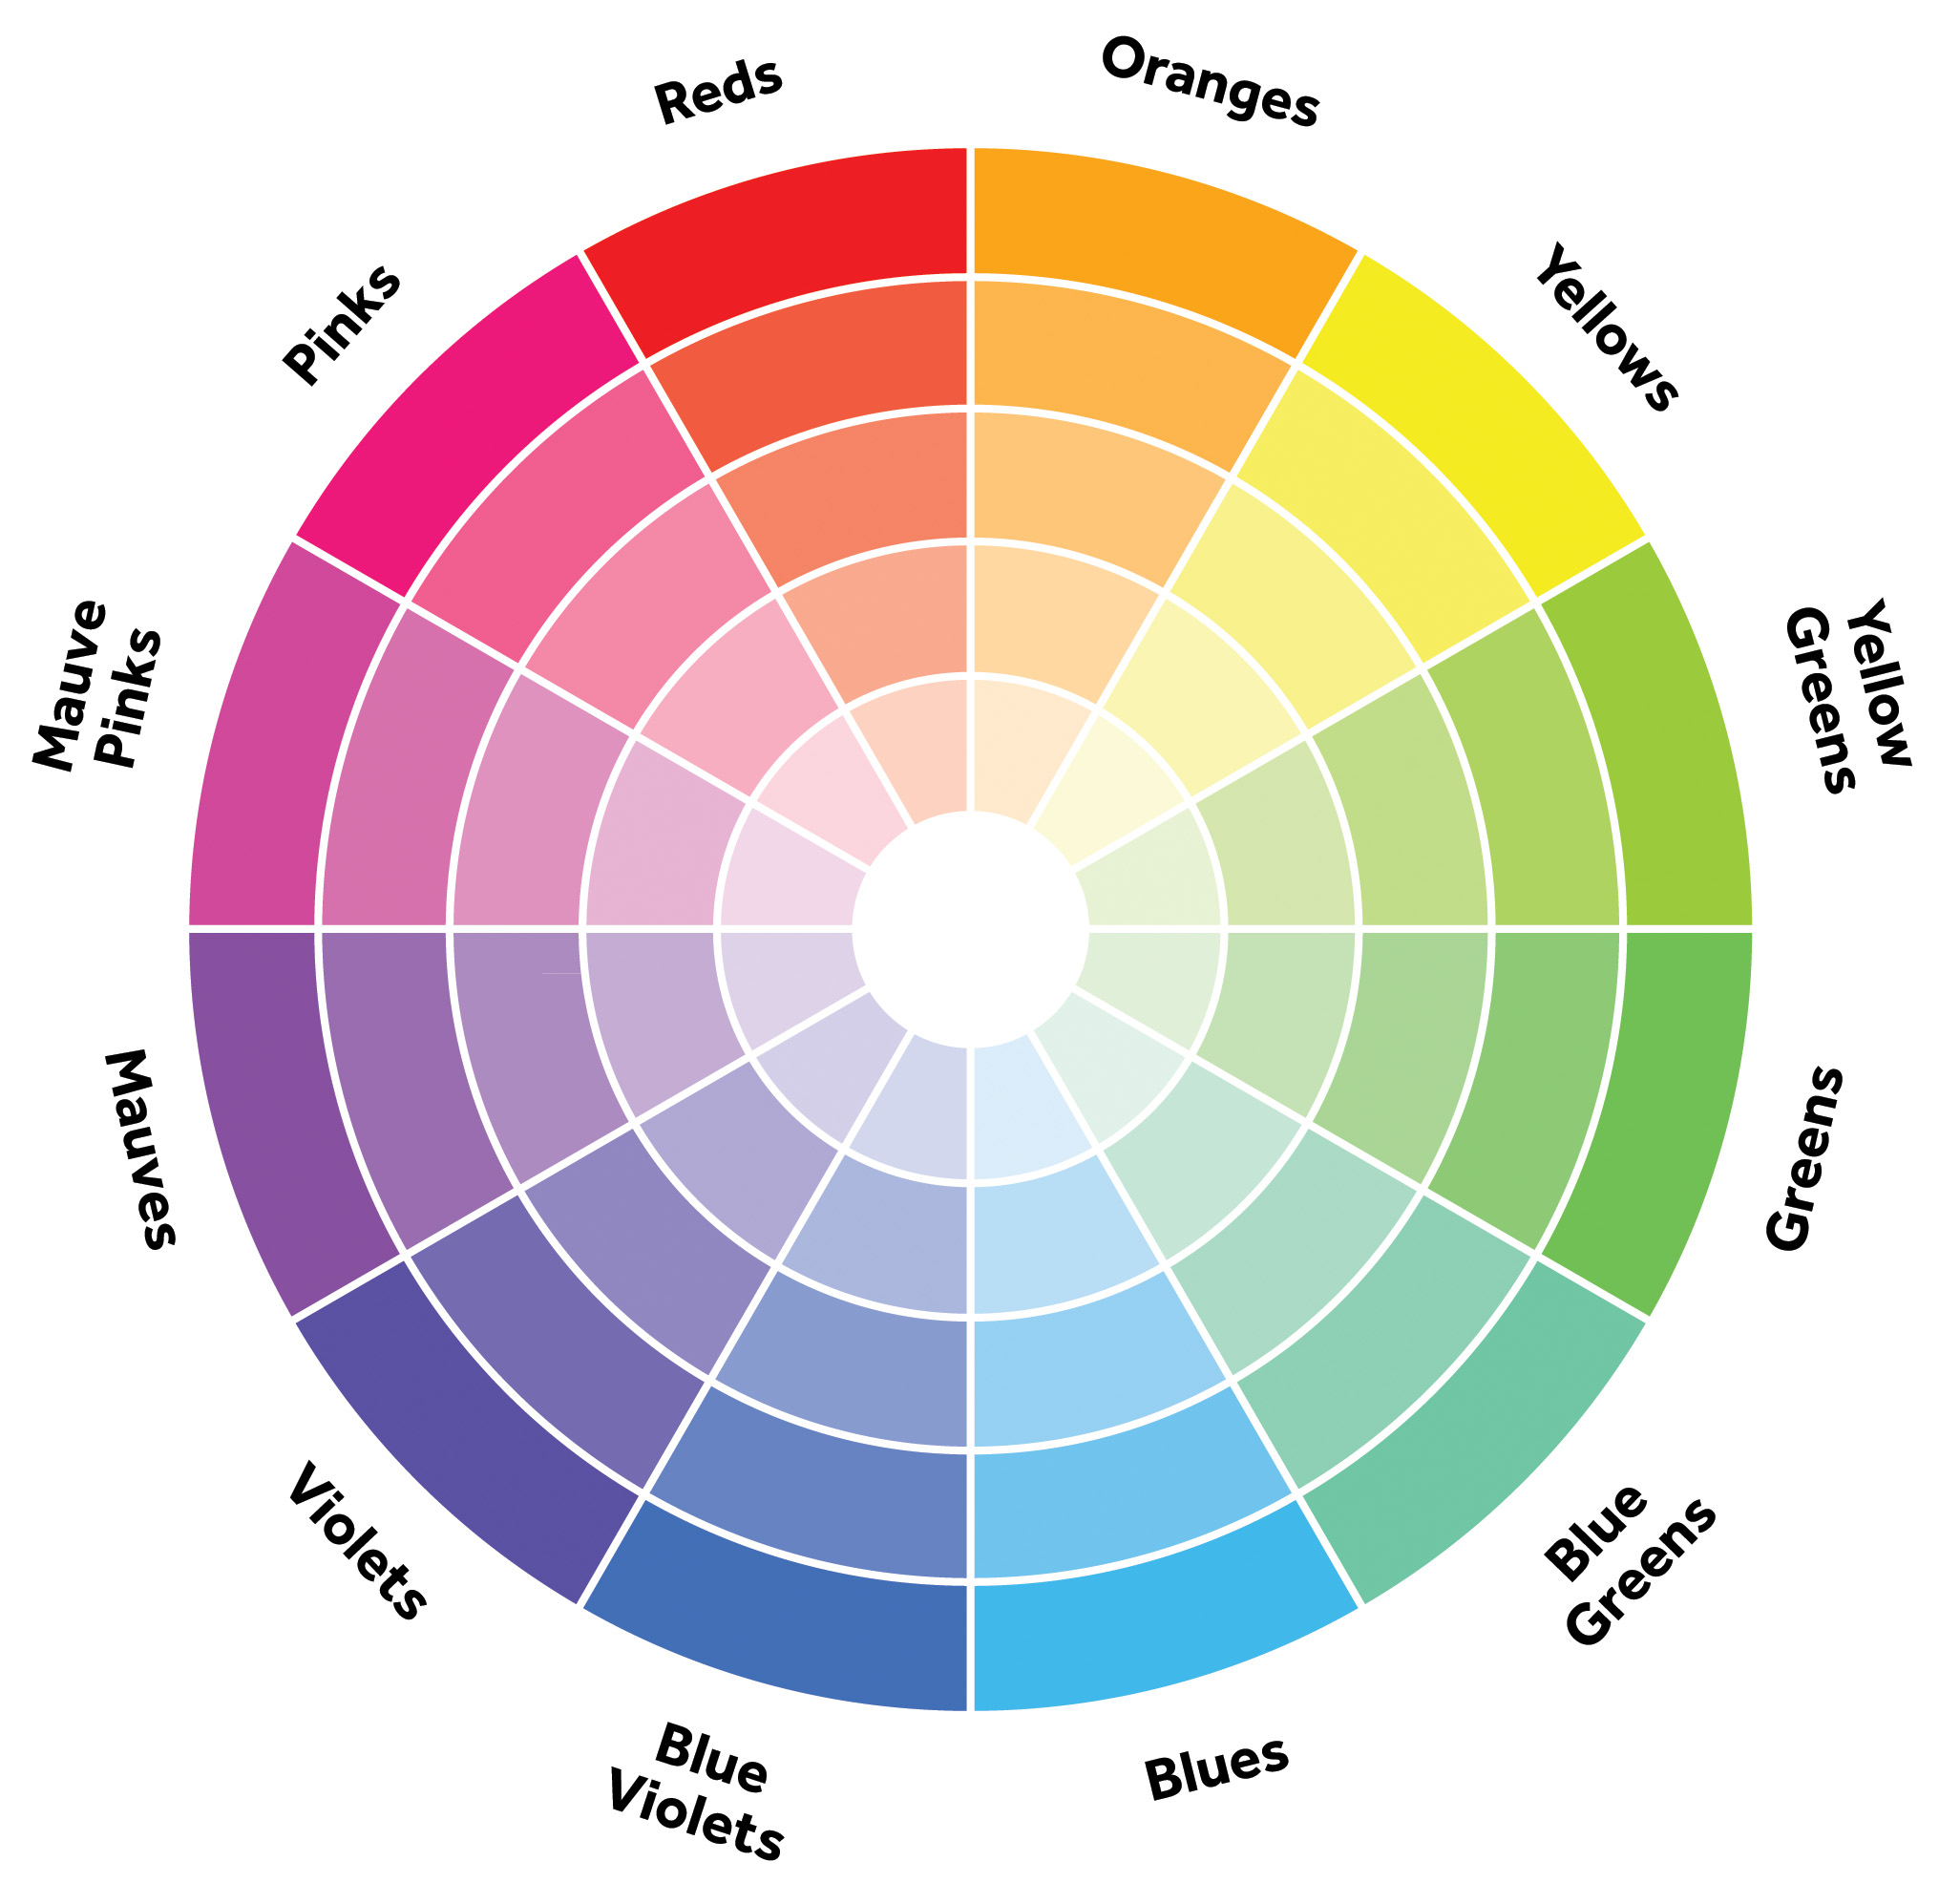
\includegraphics[scale=0.1]{color_wheel.jpg}
\caption{\label{fig:perceptron}Colour Wheel Diagram}
\end{figure}




















